\evenchapter{Diagnostic de la base de donnée topographique et cadre de travail}

\textit{Les produits cartographiques maintenus par la DAF sont les données sur lesquels porte le travail de ce stage. Cette partie s'attarde donc à les présenter et à les expliciter. La notion de généralisation et son cadre d'utilisation est elle-aussi précisée.}
 
\section{La cellule topographie de la Direction des Affaires Foncières}

\subsection{Organisation de la cellule topographie}
La cellule topographie est une cellule de la section Cadastre-Topographie qui est l'une des quatre sections de la Direction des Affaires Foncières de la Polynésie Française. Les grandes missions de ce service sont équivalentes à celles de l'IGN en métropole avec la cartographie de la Polynésie Française, l'acquisition des données ainsi que la maintenance et la densification des réseaux géodésiques et de nivellement. Ces missions sont assurées par des géomètres-cartographes et des géomaticiens qui travaillent au sein de cette cellule. 

\subsection{Produits cartographiques maintenus}
La section topographie propose de nombreux produits et prestations qu'il est possible de passer en revue dans un catalogue dédié. Il est disponible sur le site internet de la DAF [https://www.service-public.pf/daf/]. Parmi les produits cartographiques, on trouve notamment :

\begin{itemize}
\item \textbf{Des cartes et des plans } - Deux types de cartes sont proposées. La première catégorie est celle de la carte topographique de référence ( la carte au 1/5000 couvre Tahiti en 81 planches) . A Tahiti, des éditions au 1/2000 sont également disponibles sur la zone urbaine. La seconde catégorie est la carte de type \textit{CARTO ILE} avec des éditions aux 1/25000 ou 1/50000 produites sur demande en cartes papier et en dalles au format numérique jpg géoréférencé sans toutefois que les couches qui composent ces cartes ne soient réellement généralisées.
\item \textbf{Des données topographiques} parmi lesquelles on retrouve une BD Topo administrée par le SGBD PostGreSQL/PostGIS  et dont l'architecture fait l'objet de la sous-partie suivante. Les données sont en libre accès comme c'est le cas pour les produits MNT.
\item \textbf{Des photoplans et spatio-cartes} produites à partir des photographies aériennes et des photos d'archives dont la section topographie est détenteur d'une vaste collection.
\end{itemize}

Par ailleurs, une mission de ce service est la maintenance d'un vaste réseau de repères géodésiques et de nivellement utilisables par les entreprises qui peuvent avoir accès aux fiches signalétiques des repères.


\subsection{Méthodes d'acquisition de la donnée}
La création de l'ensemble de ces produits cartographiques se fait principalement par prise de vue aérienne ou satellitaire et est soumise à des obstacle météorologiques. En effet, la présence de nuage quasi-permanent en zone montagneuse rend les acquisitions difficiles. Seules certaines périodes de l'année et à des horaires bien précis sont propices aux prises de vue.  On constate cela notamment en comparant les MNT mondiaux à ceux réalisés par la section Topographie. La figure \ref{ombrage} le démontre particulièrement sur les sommets montagneux où les données d'Esri sont incomplètes en raison de la forte couverture nuageuse.
\begin{figure}[ht]
\centering
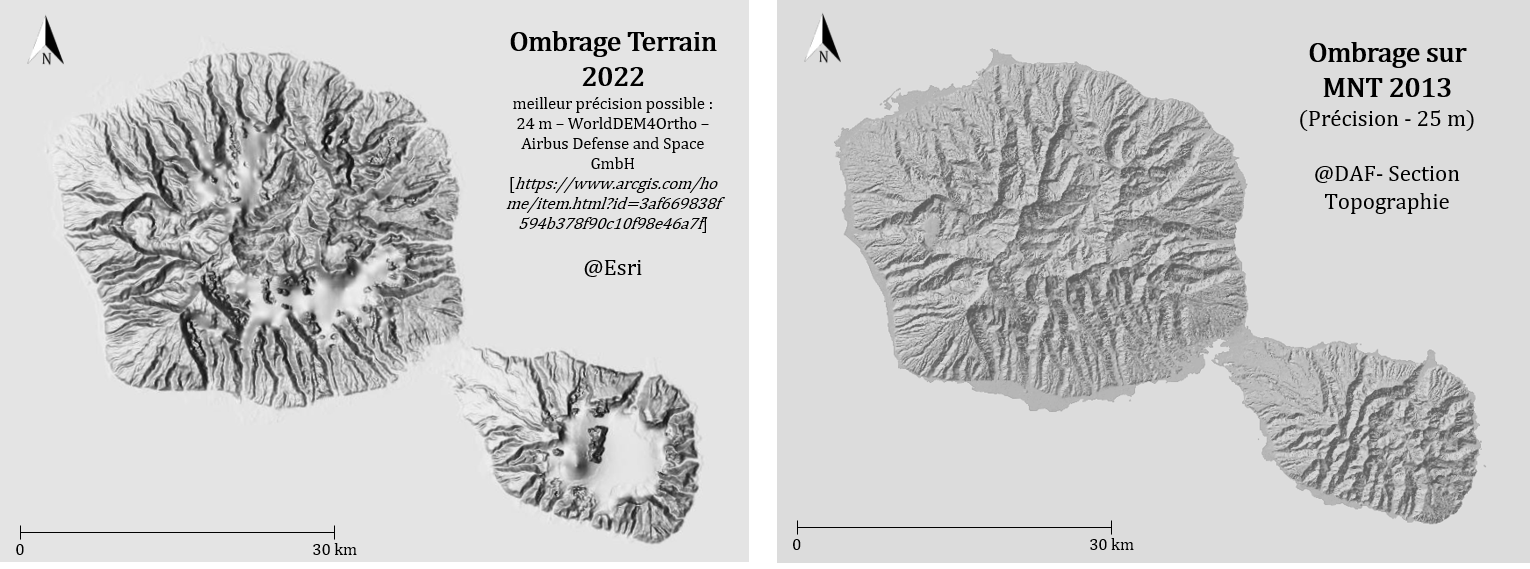
\includegraphics[width=\linewidth]{images/chap0/ombrage}
\caption{Comparaison des ombrages issus de deux sources différentes - Tahiti}
\label{ombrage}
\end{figure}

\section{Architecture de la base de données topographique de la Polynésie Française}

\subsection{Classes d'entités composant la base}

\begin{figure}[ht]
\centering
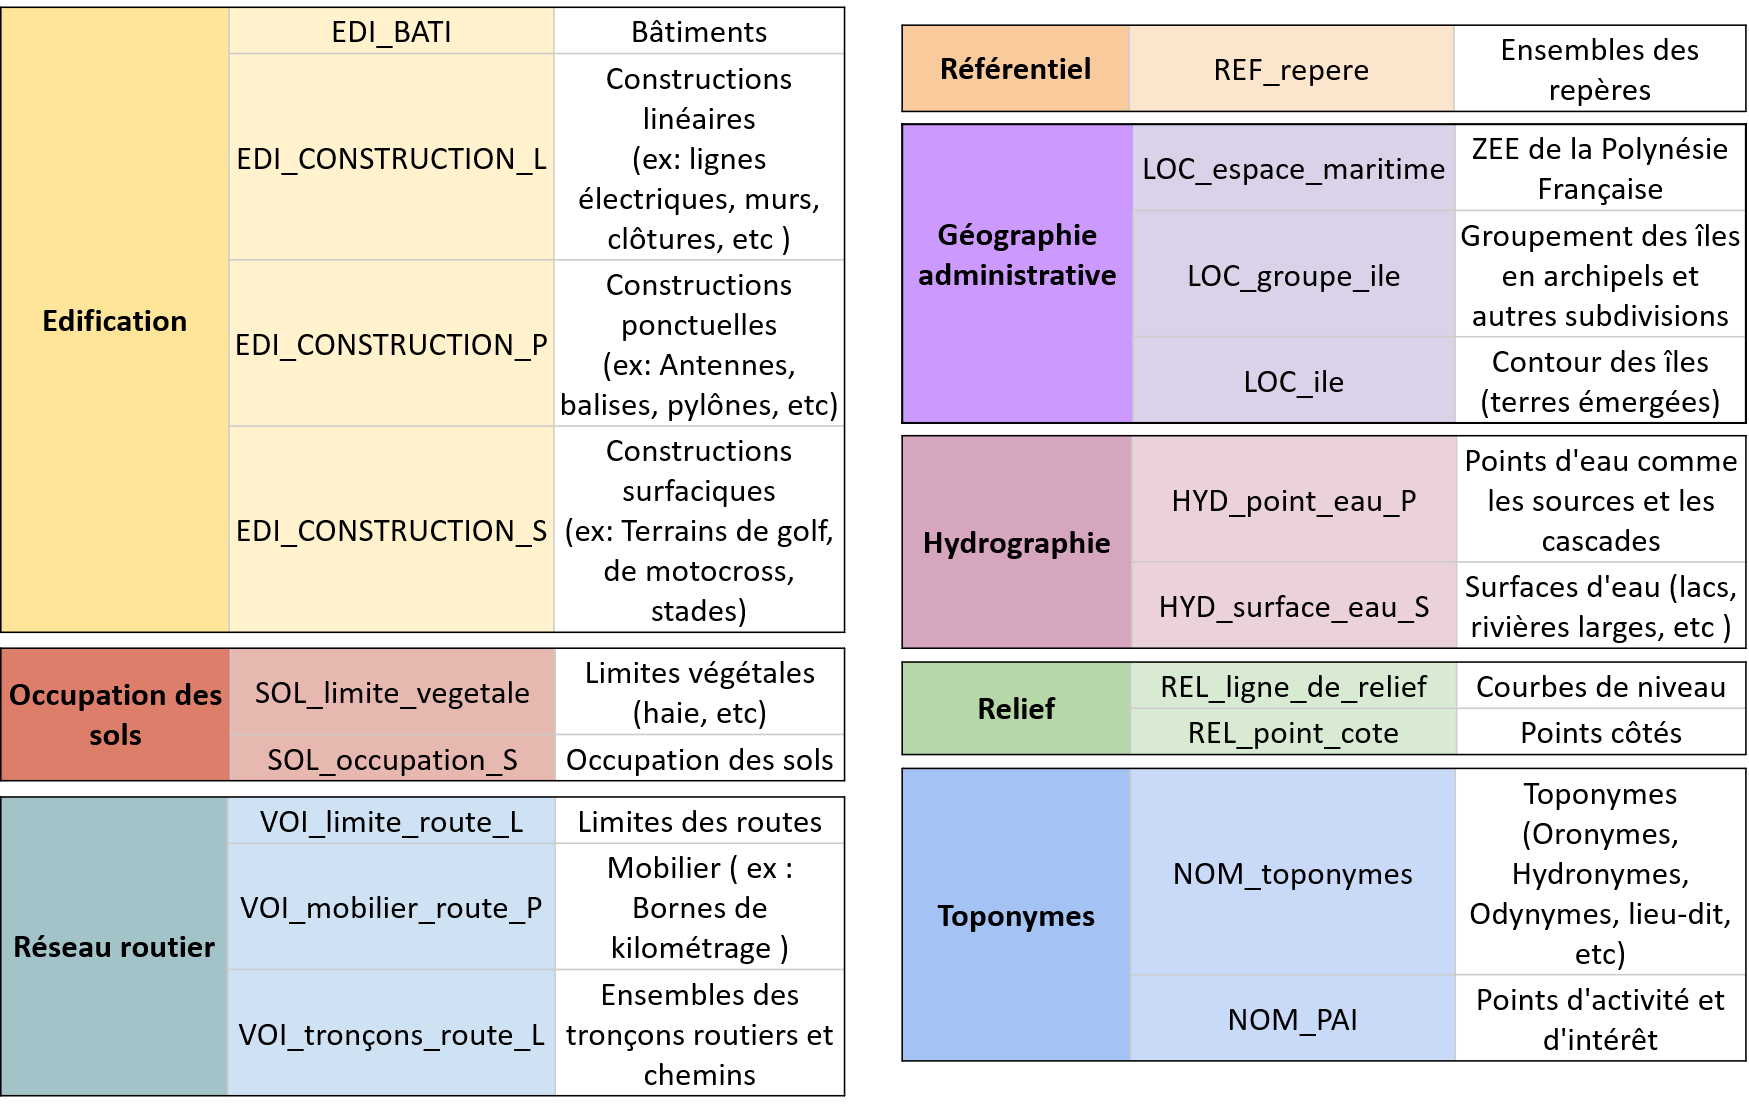
\includegraphics[width=12cm]{images/chap1/bd_simplifie.png}
\caption{Représentation simplifiée de la base de donnée de la DAF - Liste des classes du diagramme de classe la schématisant (groupement par thématique)}
\label{bd_simplifie}
\end{figure}
Les données produites par la DAF et servant à la cartographie figurent dans une base de donnée mise à jour régulièrement. C'est une \textit{base de donnée géographique}. Ce terme sera précisé dans le chapitre suivant. En effet, nous distinguerons les différentes généralisations possibles ainsi que les différents types de bases de données qui en découlent. 

De nombreux objets sont répertoriés dans la base qui s'articule en 31 classes. La figure \ref{bd_simplifie} présente une représentation schématique et simplifiée de la base de donnée faisant figurer uniquement les classes qui participent directement à la production des cartes. Une liste plus détaillée de l'ensemble des classes avec leurs détails fait l'objet de l'annexe B tandis que le diagramme UML complet de cette base de donnée figure en annexe A. On y retrouve l'ensemble des classes avec notamment les catégories et sous-catégories pour chacune d'entre elles. Pour celles qui présentent une représentation graphique, cette catégorisation est à l'origine de la symbologie.

\subsection{Répartition en quatre fuseaux UTM}
{\color{magenta} NON REDIGE : Explication de la séparation de la base en 4 fuseaux UTM + carte à mettre représentant ces fuseaux (ici ou en annexe en fonction de la place)}

\begin{figure}[ht]
\centering
\includegraphics[width=\linewidth]{images/chap0/PF_carte_generale_UTM_90x90_2012-1.png}
\caption{Carte des fuseaux UTM - Produit de la section topographie - 2012}
\label{fuseauUTM}
\end{figure}

\section{Pré-requis pour la généralisation }
\textit{L'objectif de ce travail est donc de produire des cartes qui seront réalisées avec l'outil ArcGIS. Pour parvenir à réaliser une carte multi-échelles, des traitements de généralisation doivent être effectués sur chaque gamme d'échelle. Cette sous-partie précise le terme de généralisation cartographique ainsi que les ensembles de définition choisies pour ce projet.}
\subsection{Généralisation cartographique}
Il est nécessaire de commencer ce rapport en précisant certains adjectifs qui peuvent qualifier une base de données. La base de données de la DAF dont le diagramme de classe (annexe ??) a été présenté précédemment est une \textbf{base de données géographique} Comme le fait Marion Dumont \cite{Dumont2018}, nous ferons la distinction dans ce rapport entre une base de données géographique (BDG) et une base de données cartographique (BDC) dont l'utilisation est exclusivement liée à la représentation graphique. De plus, nous distinguerons \textit{la généralisation de modèle} visant à restructurer la BDG, la \textit{généralisation graphique} visant simplement à "respecter les contraintes de lisibilité" et enfin la généralisation cartographique. La généralisation cartographique, le coeur du travail durant ce stage, est le processus qui permet de produire des cartes à différentes échelles à partir de la BDG. La figure \ref{dumont} issue de la thèse de Marion Dumont permet comprendre ces termes.

\begin{figure}[ht]
\centering
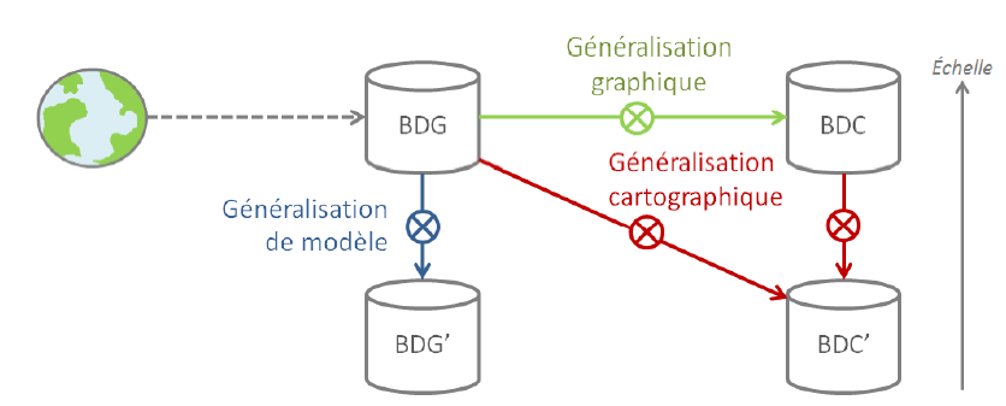
\includegraphics[width=\linewidth]{images/chap1/generalisation_dumont.png}
\caption{Les différents types de généralisation}
\label{dumont}
\end{figure}
Disposant à la fois de la base de donnée BD TOPO de la DAF ainsi que du projet type de cartographie à l'échelle 1/5000, il s'agira donc de mettre en place des traitements permettant de réaliser la cartographie non plus seulement au 1/5000 mais à des échelles inférieures. Par ailleurs le choix des échelles de travail, effectué en début de stage sera justifié plus loin.

L'objectif est d'obtenir un panel de cartes aux échelles choisies. Le travail préliminaire à la diffusion web se décompose en deux phases qui font chacune l'objet d'un chapitre de ce rapport. La première partie est une généralisation cartographique accompagnée de la production des métadonnées associées. Pour chacune des échelles, la BDG de départ sera adaptée pour fournir une BDC en accord avec l'échelle (notée BDC' sur la figure 1.4). Ensuite, le travail se poursuivra pour réaliser la cartographie à partir de cette base de donnée. L'étiquetage, l'habillage de la carte avec des fonds rasters et le choix de la symbologie feront l'objet de cette partie. Il faut noter que la première phase amènera à discuter de la structure de la BDG, que ce soit la pertinence de certains champs ou encore la nécessité d'en créer de nouveaux.

%Enfin, bien qu'il ne s'agisse que d'un travail préparatoire qui a vocation à évoluer, la perspective de la diffusion web doit être envisagée dès les premiers traitements. 

%Aux conseils du maître de stage, s'ajoutent les recommandations trouvées dans les travaux de Marion Dumont \cite{dumont}. En effet sa thèse évoque la généralisation et la fluidification des transitions entre les différents niveaux de zoom.

Au regard de cette analyse, de nombreuses questions surviennent notamment quant au choix des échelles et de la zone de travail.

\subsection{Choix des échelles}
Durant ce stage, la généralisation s'est portée sur huit niveaux d'échelle. La plus grande échelle\footnote{La question d'échelle est au coeur du processus de généralisation, et dans ce rapport, nous utiliserons souvent les termes "grande échelle" ou "petite échelle". Ils  seront employés dans leur sens arithmétique. Ainsi, l'échelle 1/5000 du cadastre est une plus grande échelle que l'échelle 1/500 000 car le dénominateur du quotient est plus faible et donc la fraction est plus grande. C'est cette convention qui est notamment utilisée par ArcGIS dans la documentation. L'ENS Lyon et sa plateforme GéoConfluence propose une définition plus détaillée de l'utilisation du terme échelle en géographie }, le 1/5000 est déjà cartographiée. Un projet ArcGIS nommé \textit{"export\_topo\_5000"} a été fourni en début de stage. Ce projet comporte l'ensemble des couches utilisées, la symbologie et l'étiquetage adéquat pour cette échelle ainsi que les fonds raster ajoutés au projet. Il sert de modèle et le travail sera fait de manière à ce que l'utilisateur puisse zoomer progressivement et naturellement vers cette carte.\\ \\ Les différents niveaux d'échelles sont :

\begin{itemize}
    \item \textbf{1/5000} (pas de traitement projet déjà réalisé)
    \item \textbf{1/10000}
    \item \textbf{1/15000}
    \item \textbf{1/25000} (échelle de référence pour la carte de randonnée)
    \item \textbf{1/50000}
    \item \textbf{1/100000} (échelle idéale pour visualiser Tahiti entièrement au format A0) 
    \item \textbf{1/250000} (échelle idéale pour visualiser Tahiti & Moorea entièrement au format A0)
    \item \textbf{1/500000}  (échelle idéale pour visualiser les îles du vent entièrement au format A0)
\end{itemize}
\vspace{0,3cm}
Cette échantillon permet de s'adapter au mieux aux échelles d'ArcGIS et donc à la vocation future de diffuser ces cartes sur le web. La contrainte  d'utiliser des échelles bien précises (comme le 1/25000 par exemple) se justifie par le fait que ce travail de cartographie pourrait être utilisé des demandes de cartes en papier et notamment à cette échelle qu'on peut qualifier \textit{d'échelle critique} ou \textit{de point de généralisation} selon la définition de \cite{Ratajski_1967} car "un changement important de représentation est nécessaire".

\subsection{Choix de la zone de travail}

En ce qui concerne la zone de travail, la priorité reste la cartographie des deux îles principales Tahiti et Moorea. L'importance de ces deux îles se mesure non seulement par leur superficie de terre émergée mais aussi par la concentration d'activités et de population et donc par conséquent, par l'importance des éléments cartographiques qui en découlent. En cartographiant Tahiti, il est donc plus probable de voir apparaître certains défauts de cartographie permettant de faire les ajustements nécessaires. C'est seulement à la fin du stage, et dans un temps restreint, que les traitements seront appliqués sur les données des autres îles.
Comme cela a été illustré dans le chapitre précédent, les données vecteurs de la DAF sont séparées en 4 fuseaux et Tahiti et Moorea font partie du fuseau 6. C'est sur ce fuseau que seront réalisés les traitements en priorité puis généralisés ensuite aux autres fuseaux (5, 7 et 8). Enfin, les fonds raster, produits île par île, ne seront ajoutés que sur les deux îles principales\footnote{Dans le cadre de la diffusion du portail web, la diffusion de fonds raster s'avère difficile et coûteuse. Cette problématique est évoquée dans la troisième partie du rapport concernant la diffusion web.}.


